\chapter{Introduzione}

%%%%%% OBIETTIVI %%%%%%%%
\section{Obiettivi del progetto}

Questo progetto di tesi si pone l’obiettivo di trovare delle relazioni tra
diversi indici bibliometrici che vengono utilizzati  per valutare la produzione
accademica. Una visione complessiva dei dati può essere utile per valutare gli
andamenti e migliorare la produttività accademica. L’applicazione sviluppata
permette, tramite interfaccia grafica, di gestire e visualizzare autori, paper,
università e conferenze, interfacciandosi con un database per l’inserimento e
l’interrogazione dei dati.

L'analisi di tali indici si concentra principalmente su quelli derivati da conferenze,
descritte in Sezione~\ref{sec:conferenze}.

%%%%%% CONTESTO %%%%%%%%%

\section{Contesto}


Nell’ambito della pubblicazione di testi di interesse accademico, una
\textit{pubblicazione scientifica} è definita come uno scritto oggettivo
riguardante un argomento scientifico, redatto da ricercatori o gruppi di ricerca
universitari.

Il gruppo di ricerca rende ufficialmente pubblici i metodi e i risultati delle
proprie ricerche sottoponendo il paper ad una conferenza oppure pubblicandolo
su riviste accademiche. Le pubblicazioni sono regolamentate da procedure di
accettazione e valutazione per stabilire se il lavoro presentato possieda i
requisiti per essere pubblicato.

\subsection{Criteri e classificazioni di pubblicazioni scientifiche}

Le pubblicazioni scientifiche vengono suddivise dal Ministero dell'Istruzione,
dell'Università e della Ricerca in una serie di categorie
\cite{criteri2009pubblicazioni}, che sono:

\begin{itemize}
    \item Gli \textit{articoli pubblicati su riviste scientifiche}, che
    riportano un codice ISSN e che sono stati  sottoposti a una procedura di
    revisione prima della pubblicazione per garantire autorevolezza;
    \item Le \textit{monografie di ricerca} che riportano codice ISBN e hanno
    superato la procedura di  accettazione per la pubblicazione;
    \item Gli \textit{articoli pubblicati in volumi collettivi}, sottoposti
    anch'essi alle stesse procedure di  accettazione degli articoli pubblicati
    su riviste scientifiche;
    \item Tutto ciò che sia riconducibile ad attività di ricerca, come brevetti, software, disegni, 
    purché accompagnati da pubblicazioni e documentazione per poter essere valutati.
\end{itemize}
%
Questi non risultano essere però l'unica classificazione esistente. Un altro
esempio di classificazione, seppur molto simile, è visibile in~\cite{oechsner2013}.

Inoltre, il MIUR ha anche proposto quattro criteri che devono essere
simultaneamente soddisfatti affinché un certo documento possa essere definito
come ``pubblicazione accademica'' \cite{criteri2013pubblicazioni}.
Essi sono:

\begin{itemize}
    \item I risultati presentati devono essere originali;
    \item I risultati presentati devono poter essere verificati e riutilizzati
    in altre attività di ricerca;
    \item Il linguaggio deve rendere la pubblicazione accessibile alla maggior
    parte delle persone interessate;
    \item La sede editoriale deve assicurare l’esistenza di una \textit{peer review} esterna.
\end{itemize}

Oltre a tali criteri, considerati di carattere generale, lo stesso
documento~\cite{criteri2013pubblicazioni} propone altri proprietà specifiche per
pubblicazioni e riviste scientifiche.

In particolare, una \textit{pubblicazione} può considerarsi scientifica se
espone in modo sistematico i risultati originali del lavoro di ricerca facendo
uso di riferimenti bibliografici, in modo tale che possano essere verificati da
terzi e riutilizzati in altre attività di ricerca.
Dev'essere inoltre sottoposta ad una procedura di revisione ed essere disponibile
in biblioteche universitarie o pubblicamente.

Diversamente, una \textit{rivista} è considerata scientifica se aderisce ai criteri
generali elencati prima, la revisione è formalizzata ed anonima, e garantisce una
periodicità nelle sue uscite.

\subsection{Struttura di una pubblicazione}

Una pubblicazione deve necessariamente presentare i seguenti campi:
\begin{itemize}
    \item \textit{Titolo}: deve fornire un riassunto di ciò che viene trattato
    nell'articolo;
    \item \textit{Nomi degli autori}: solitamente viene elencato seguendo
    l'ordine alfabetico oppure indicando il nome del ricercatore che ha
    contribuito maggiormente alla ricerca;
    \item \textit{Abstract}: un sommario per descrivere gli aspetti fondamentali
    del lavoro;
    \item \textit{Parole chiave}: lista di parole che si riferiscono agli
    argomenti trattati nell'articolo;
    \item \textit{Classificazione tematica};
    \item \textit{Introduzione}: breve paragrafo che indica gli scopi della ricerca;
    \item \textit{Metodi}: modi in cui sono stati condotti gli studi, i quali
    è fondamentale che usino procedure scientifiche, riproducibili da chiunque
    e confutabili;
    \item \textit{Risultati}: elenco dei dati scientifici ottenuti;
    \item \textit{Discussione}: interpretazione e analisi oggettiva dei dati;
    \item \textit{Conclusione}: considerazioni ed epilogo del lavoro svolto;
    \item \textit{Riferimenti}: elenco delle note bibliografiche;
    \item \textit{Riconoscimenti, appendici e supplementi}: informazioni accessorie.
\end{itemize}

\subsection{Conferenze scientifiche}\label{sec:conferenze}
\label{sec:conferenze_scientifiche}

Una conferenza scientifica è un evento al quale i ricercatori prendono parte per presentare e discurere i propri lavori accademici. Le conferenze sono un modo per scambiarsi informazioni, ricevere feedback da altri ricercatori, stabilire nuovi contatti e avviare nuove collaborazioni. 
Tra i vari incontri, si fa solitamente una distinzione in termini di grandezza: il più grande prende il nome di conferenza, altrimenti viene chiamato workshop.

Tipicamente, le conferenze scientifiche si dividono in tre categorie: 
\begin{enumerate}
    \item Piccoli convegni organizzati intorno al tema principale;
    \item Conferenze generali con un focus più ampio e vari argomenti, solitamente organizzate a livello nazionale o internazionale e che si tengono periodicamente una volta l'anno;
    \item Conferenze professionali di grandi dimensioni, non limitate solo all'ambito accademico ma anche a problemi correlati.
\end{enumerate}

La differenza tra un documento presentato ad una conferenza rispetto ad uno
presentato ad una rivista di ricerca è che il primo è più breve e i tempi
di revisione sono minori. Il lavoro inviato alle conferenze è, generalmente,
limitato alla pubblicazione all’interno della documentazione della conferenza.
Ciononostante, in caso di ottimi lavori, essi possono essere estesi per una
futura pubblicazione su riviste scientifiche.

I ricercatori vengono invitati ad approfondire i temi attuali tramite le
\textit{call for papers} (CFP), che di solito includono il tema e lo scopo della
conferenza, le linee guida per le presentazioni, i requisiti per le proposte
e le scadenze da rispettare. Quando si sottopone un paper ad una conferenza,
bisogna tener presente che il pubblico a cui ci si riferisce è molto specifico;
perciò, la presentazione dell’elaborato deve essere unica, adattata al tema e
allo scopo della conferenza.

% Prima di sottomettere il paper alla conferenza è necessario scrivere una
% proposta per l’articolo. È una breve presentazione, simile ad un abstract, che
% deve tenere conto dei requisiti unici per la conferenza. Se la presentazione
% del paper verrà accettata, sarà possibile presentare il proprio lavoro alla
% conferenza.

Un indice importante che riguarda le conferenze è il \textit{rating}, cioè
come viene valutata una conferenza. In questo progetto di tesi si è tenuto
conto del rating fornito dal GGS.

L'iniziativa GGS è data dall'unione di tre membri: GII, GRIN e SCIE che si sono prefissi l'obiettivo di elaborare una classificazione delle conferenze di informatica, combinando approcci bibliometrici e non.

Il GII (Gruppo di Ingegneria Informatica) \cite{gii} ed il GRIN (Gruppo di Informatica) \cite{grin} sono dei gruppi di ricercatori universitari con l'obiettivo di organizzare e promuovere le attività scientifiche in Italia. Anche la SCIE (Sociedad Científica Española de Informática) svolge un ruolo simile, ovvero la promozione dell'informatica, in Spagna.

La classifica \cite{ggsRatingPdf} si basa sulla combinazione ponderata tra classifica CORE e altre fonti. Inoltre, l'algoritmo utilizzato applica un passo di normalizzazione, ottenuto dividendo il numero di citazioni e il numero di pubblicazioni, ad ogni conferenza.
Si ottiene quindi la classifica visibile in Tabella \ref{table:ratings}.
Notare che in questa tabella manca il rating \textit{C}, che viene riservato
dal CORE per le conferenze al di sotto di quelle con rating \textit{B}.
Per quanto riguarda in particolare l'ambito di ricerca in sicurezza informatica,
ci sono quattro conferenze considerate \textit{top}. Esse sono CCS, S\&P, Usenix
e NDSS.

\begin{table}
    \centering
    \begin{tabular}{||c c ||} 
     \hline
     Classe & Descrizione \\ [0.5ex] 
     \hline\hline
     A++, A+ & Conferenze di ottimo livello \\ 
     \hline
     A, A- & Conferenze di alto livello \\
     \hline
     B, B- & Conferenze di buon livello \\
     \hline
     Work In Progress & Rating non ancora calcolato \\
     \hline
    \end{tabular}
    \caption{Rating delle conferenze}
    \label{table:ratings}
\end{table}

Il CORE (Computing Research and Education Association of Australasia), invece, valuta i dati sottomessi dalle conferenze, considerando:
\begin{itemize}
    \item L'insieme delle citazioni del lavoro, basandosi su dati provenienti da Google Scholar, Elsevier e le citazioni dei paper più influenti; 
    \item Quanti ricercatori di rilevo sono interessati alla conferenza;
    \item Quanto è di rilievo la commissione di programma, basandosi sull'$h$-index di Elsevier;
    \item Il livello di accettazione dei paper che, se elevato, può essere un indicatore negativo.
\end{itemize}

A causa di un numero limitato di ricercatori internazionali coinvolti nella presentazione e nella valutazione degli elaborati, la copertura delle conferenze di informatica non è completa e il CORE considera circa mille conferenze, a fronte delle 5800 di DBLP.

%%%% SCOPUS %%%%

\subsection{Scopus}\label{sec:scopus}

Scopus~\cite{scopus} è una base di dati sviluppata da Elsevier che contiene
papers e articoli che riguardano la ricerca in ambito scientifico, tecnologico,
biomedico e delle scienze sociali. Il database viene aggiornato quotidianamente
ed è possibile consultare articoli a partire dal 1966. Inoltre permette
all'utente, collegato ad una rete universitaria, di accedere velocemente agli
abstract e ai testi completi.
I dati utilizzati per la costruzione del database di questo progetto di tesi sono stati scaricati per la maggior parte da Scopus. 

Alcuni indicatori registrati da Scopus per gli autori sono:
\begin{itemize}
    \item \textit{Citation count}, che indica il numero di volte in cui le
    pubblicazioni di un autore sono state citate in altri articoli di riviste
    trattate da Scopus;
    \item \textit{Cited-by count}, un indice di citazione a livello di articolo,
    indica quante citazioni sono state ricevute. Questo indicatore viene
    utilizzato anche per articoli scientifici e il conteggio viene riportato
    accanto al riferimento bibliografico;
    \item \textit{$h$-index}, un indice che misura la produttività e l'impatto che
    ha il lavoro pubblicato da un ricercatore.
\end{itemize}

Con riferimento all'$h$-index, esso è stato suggerito da Hirsch nel 2005~\cite{hirsch2005}
e rappresenta il numero $h$ di paper pubblicati da un certo autore che hanno
almeno $h$ citazioni. Ad esempio, se un autore ha $h$-index pari a 4, significa
che ha 4 lavori con almeno 4 citazioni.

Scopus registra anche informazioni riguardanti le varie università (o, più
in generale, affiliazioni) a cui gli autori appartengono. Alcuni indicatori
registrati a tale fine sono:
\begin{itemize}
    \item \textit{Numero degli autori} che pubblicano per l'università;
    \item \textit{Numero dei documenti}, che riguarda il numero di paper prodotti dall'università.
\end{itemize}


%%% GOOGLE SCHOLAR %%%
\subsection{Google Scholar}\label{sec:google-scholar}

Google Scholar~\cite{scholar} è un motore di ricerca web gratuito che indicizza il testo
completo (o i metadati) di letteratura scientifica in varie discipline.

Google Scholar include articoli di riviste, libri, conferenze, tesi, abstract,
report tecnici e così via.
Mentre Scopus è una base di dati aggiornata quotidianamente da Elsevier, Google
Scholar fa uso di \textit{web crawlers} per scoprire in modo automatico nuovi
articoli e ricavare senza intervento umano la rete di citazioni.
Una prima statistica del 2014~\cite{khabsa2014} stima che Google Scholar
indicizzi fra il 79\% ed il 90\% della letteratura scientifica in inglese,
per un totale di 100 milioni di articoli.

A differenza di Scopus, Google Scholar non offre una API ufficiale per l'accesso
programmatico agli articoli che indicizza~\cite{stackoverflowScholarAPI}: per
questo motivo non è stato usato come fonte dei dati usati in questa tesi.




%%% MODELLIZZAZIONI %%%%%
\section{Modellizzazioni}\label{sec:modellizzazioni}

Nella modellazione del problema si è tenuto conto solamente dell'ambito di
paper sottoposti a conferenze. Le entità principali risultano quindi essere
le seguenti quattro:

\begin{itemize}
    \item \textit{Conference}, la conferenza a cui viene sottoposto il paper;
    \item \textit{Affiliation}, l'università per cui l'autore ha fatto ricerca. 
    \item \textit{Paper}, il paper portato alla conferenza;
    \item \textit{Author}, l'autore di uno o più paper. 
\end{itemize}

Un paper può partecipare ad una sola conferenza e può essere scritto da uno o
più autori, che possono avere affiliazioni diverse. Si viene perciò a
creare una tripla tra le entità Paper, Affiliation e Author.
%  Per semplificare
% lo schema, si è introdotta la tabella Pubblication visibile in Figura
% \ref{fig:er2}, che ha come attributi  le chiavi primarie delle tre entità
% precedenti, tenendo comunque in considerazione che un autore, su uno stesso
% paper,  può avere affiliation diverse.
Nel modello ER in Figura \ref{fig:er1} sono visibili le relazioni che
intercorrono tra le entità.

Per quanto riguarda lo schema logico ed i dettagli delle varie entità,
fare riferimento alla Sezione~\ref{sec:descrizionedati}.

\begin{figure}
    \centering
    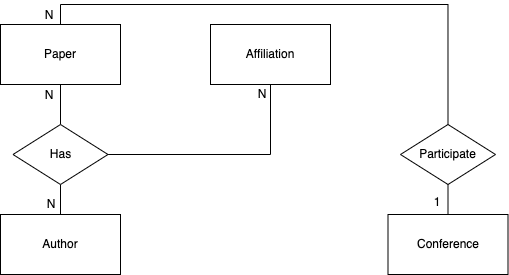
\includegraphics[width=0.8\linewidth]{er1.png}
    \caption{Modello ER del problema}
    \label{fig:er1}
\end{figure}
